%!TEX root = ../main.tex
\chapter{Introduction}\label{ch:introduction}

\section{Problem statement}\label{problemstatement}
Based on recent reports, number of smartphone subscriptions worldwide is expected to  exceed 6.1  {\em billion} mark in 2020~\cite{ericcson_report}. In the US, the use of mobile Internet has already exceeded  laptops and tablets~\cite{mobile-overtake}. For a considerable amount of users, the smartphone is the only compute device in their possession~\cite{mobile-only}. Not surprisingly, for many users, mobile pages are the primary portal for content, and mobile browsers continue to be one of the most popular applications on smartphones~\cite{charlie_mobicom2015}. However, the page load performance on mobile devices does not match up to its importance: mobile page load times are an order of magnitude slower than desktop, often taking 10s of seconds to load just the landing page~\cite{klotski}.\\

\noindent Unfortunately, it is not easy to improve mobile Web performance: several Web optimizations have been designed, but their effect on improving mobile page load times have been mixed. \\
FlyWheel~\cite{flywheel}, Google's data compression proxy, significantly reduces data usage on mobile devices, but its effect on page load time is mixed. HTTP 2.0~\cite{spdy} is known to significantly improve performance over HTTP for desktop browsers, but studies show that the improvement over mobile browsers is not significant~\cite{spydier}. Other research projects target specific aspects of the mobile browsing such as the network latency~\cite{parcel} or user QoE~\cite{klotski}, but have not been successful in improving the performance of the entire mobile page load time.

\section{Challenges}

There are three main challenges in improving mobile page load times: {\em  dependency}, {\em complexity} and {\em variances}. In order to understand challenges in improving mobile page load times, we first need to understand how the browser loads a web page.\\
\noindent So, we start with some browser background. 
\subsection{Browser Background}
Browser is a sophisticated software which comprises several interdependent activities. These activities can holistically be categorized as computation and network activities.\\
 \begin{figure}[!htb]
  \centering
    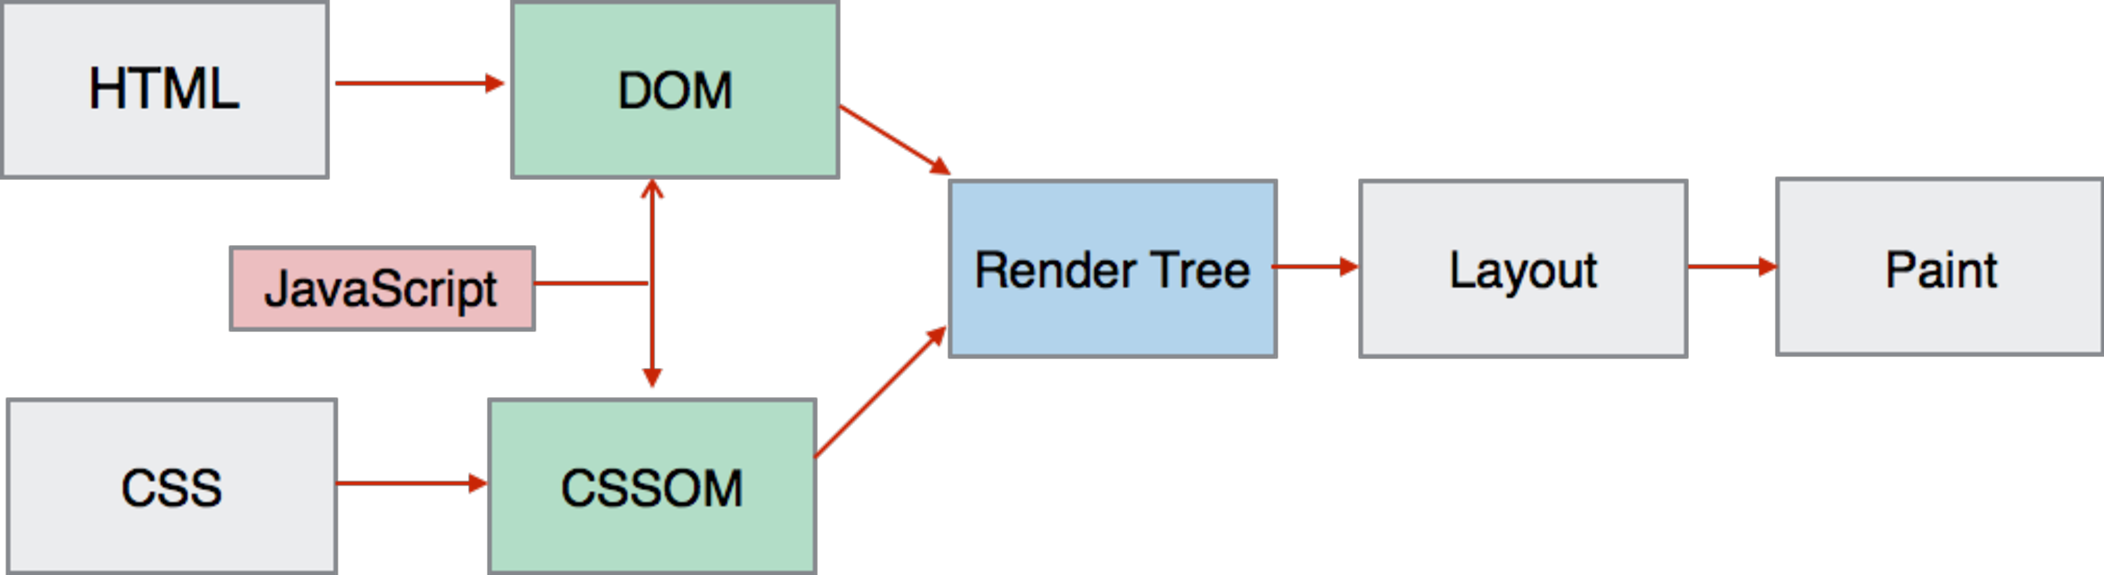
\includegraphics[width=0.85 \textwidth]{./figures/introduction/pageloadprocess.pdf}
  \caption {Page load process inside a browser}
  \label{fig:pageloadprocess}
\end{figure}

\noindent Browser starts off with fetching the html page (Figure \ref{fig:pageloadprocess}), a network activity. After receiving the first chunk of HTML page, HTML parsing process starts in parallel to generate the Document Object Model, or DOM\cite{dom}, a computation process.\\
DOM provides a structured representation of the document as a tree and it defines a way that the structure can be accessed from programs so that they can change the document structure, style and content.\\
\noindent  For example, for the sample following HTML code, first, the browser identifies HTML  {\em objects} such as {\em html}, {\em head}, {\em body} , \ldots.\\
\noindent Then, since the HTML markup defines relationships between tags, objects are connected in a tree data structure to hold the parent-child relationship from the original markup. {\em html} object is parent of the {\em body} object, the {\em body} object is parent of the {\em paragraph} object and so on.
\begin{minted}[frame=leftline, framerule=1.5pt, rulecolor=\color{blue}]{html}
<html>
  <head>
    <link href="style.css" rel="stylesheet">
  </head>
  <body>
    <p>Hello DOM!</p>
    <div><img src="d.jpg"></div>
  </body>
</html>
\end{minted}

\noindent The corrosponding DOM tree is depicted in figure \ref{fig:dom}.
 \begin{figure}[!htb]
  \centering
    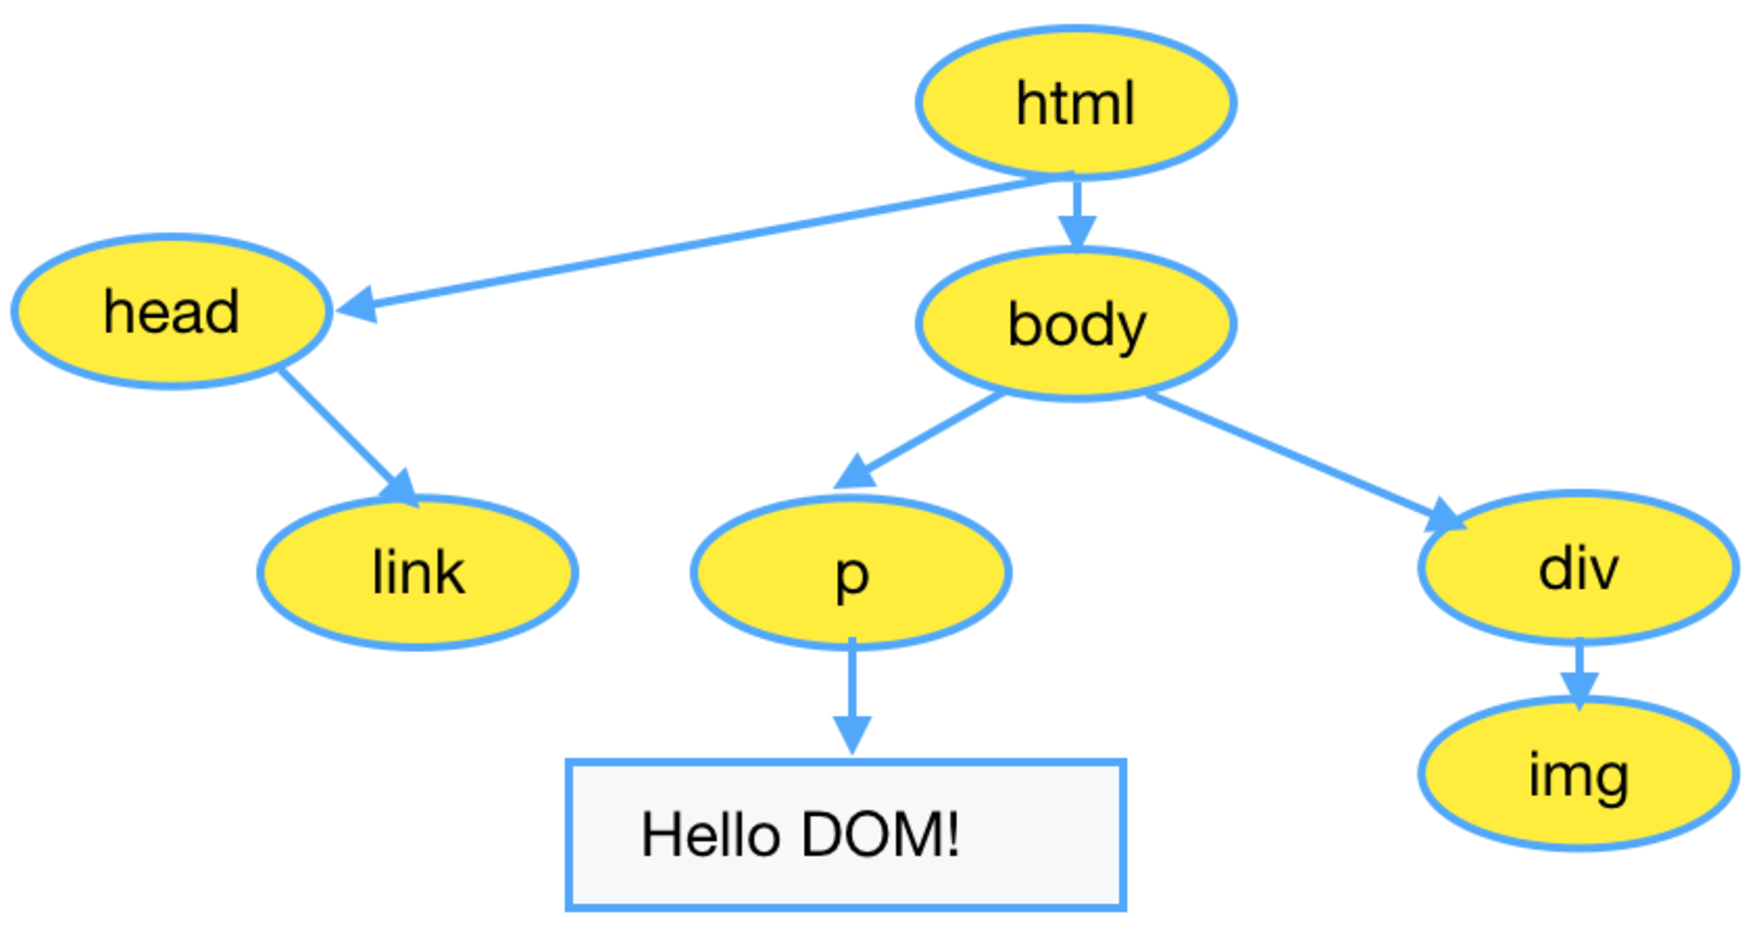
\includegraphics[width=0.85 \textwidth]{./figures/introduction/dom.pdf}
  \caption {DOM construction}
  \label{fig:dom}
\end{figure}

\noindent Rendering process also continuously renders the page, based on the intermediate DOM structure.
In rendering process, layout computes the exact position and size of each object and paint process takes in the final render tree and renders the pixels to the screen.\\

\noindent As the parsing progresses, new objects need to be downloaded based on the page's HTML code. If the object happens to be a regular Javascript (instead of asynchronous Javascript) or a CSS file, DOM construction process is blocked until these scripts are downloaded and parsed, Imposing {\em dependency} between activities.


\subsection{Dependency}
We start with {\em dependency} as the first challenge in improving page load time.
Each computation or networking elements running during the page load process is called an activity. 
As we have seen so far, activities lie in either {\em computation} or {\em networking} class. \\

\noindent From a different perspective, We can classify activities based on their dependency behavior.

\noindent There are activities that can be loaded/executed independent of  other activities\footnote{Obviously, all activities are dependent on the loading and parsing of the main html file. When we talk about activities, we are often talking about objects inside the root html file.}. \\

\noindent For example, two images in the following HTML code can be downloaded in parallel. Loading one of them does not depend on loading the other.\\ 


\begin{minted}[frame=leftline, framerule=1.5pt, rulecolor=\color{blue}]{html}
<html>
  <body>
     <img src = "a.jpg"/>
     <img src = "b.jpg"/>
  </body>
</html>
\end{minted}

\noindent In order to observe how activities are ordered in a page load process, We use WProf\cite{wprof}. WProf is discussed in \S\ref{ch:methodology}.
%WProf is a tool built atop the open source Chromium browser and is able to infer dependency policies of the browser. 
%WProf uses fine-grained timing of activities involved in a page load process to accurately extract the page {\em dependency graph} and the {\em critical path} inside such graph.
%We say an activity $a_2$ is dependent on a previously scheduled activity $a_1$ , if $a_2$ can be executed only after $a_1$ is being executed or completed. \\
%Considering activities as nodes of a graph  and inter-dependency relations as the edges of such graph, the resulting graph would be a DAG (Directed Acyclic Graph) which we call {\em dependency graph} hereafter.\\

%\noindent {\em Critical path} is the sequence of activities which add up to the longest overall duration inside the dependency graph.\\

%\noindent In addition, we use WProf-M, the mobile version of WProf for Android OS, to extract the dependency graph in a mobile environment.
\noindent For example, for the above mentioned HTML code, figure\ref{fig:twoimages} illustrates the corresponding dependency graph.\\
The X axis shows time in milliseconds and Y axis which grows from top to down, only  shows the order of objects inside an HTML file.
The light blue circle is the very first download HTML activity which is followed by a HTML evaluation activity (dark blue).
Two long purple bars refer to download of "a.jpg" and "b.jpg" ,respectively. 

 \begin{figure}[!htb]
  \centering
    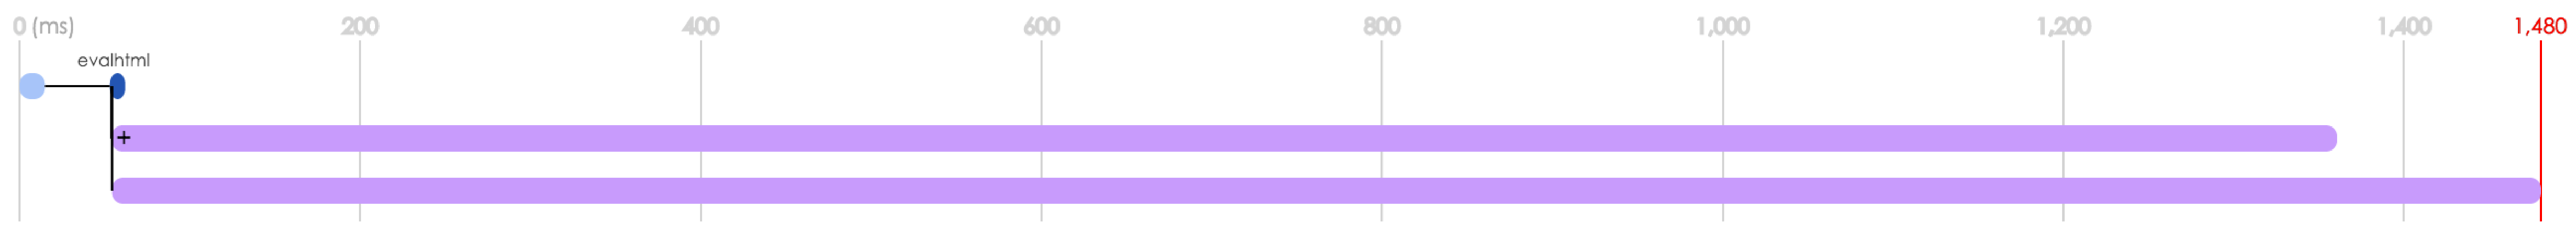
\includegraphics[width=0.85 \textwidth]{./figures/introduction/twoimages.pdf}
  \caption {Dependency graph for a HTML page with two independent images}
  \label{fig:twoimages}
\end{figure}

\noindent On the other hand, there are several activities inside a page load process that {
\em affects/will be affected} by other activities. 
For instance, adding more activities to the simple HTML code, brings about two different possible dependency scenarios:
\begin{enumerate}
  \item Adding Javascript after loading all images. 
   \begin{minted}[frame=leftline, framerule=1.5pt, rulecolor=\color{blue}]{html}
  <html>
  <body>
    <img src = "a.jpg"/>
    <img src = "b.jpg"/>
    <img src = "c.jpg"/>
    <img src = "d.jpg"/>
    <img src = "e.jpg"/>
    <img src = "f.jpg"/>
    <img src = "g.jpg"/>
    <img src = "h.jpg"/>
    <img src = "i.jpg"/>
    <script src = "b.js"> </script>
  </body>
</html>
\end{minted}
  In this case, as Javascript is loaded and executed after all images, image loading is not blocked by Javascript load, that is,  loading of images does not {\em depend} on loading of Javascript code.
  
However, there still is an internal dependency between loading the Javascript and it's execution.\\

Generally speaking, for all activities which need computation, such as HTML, Javascript, CSS, \dots  there always exists a {\em Load dependency}.
The dependency graph for this scenario is depicted in Figure\ref{fig:imagejs}\\ 
The bottom bars are showing Javascript ({\em b.js}) download and execution. They start after all images has been started.
 
 \begin{figure}[!htb]
  \centering
    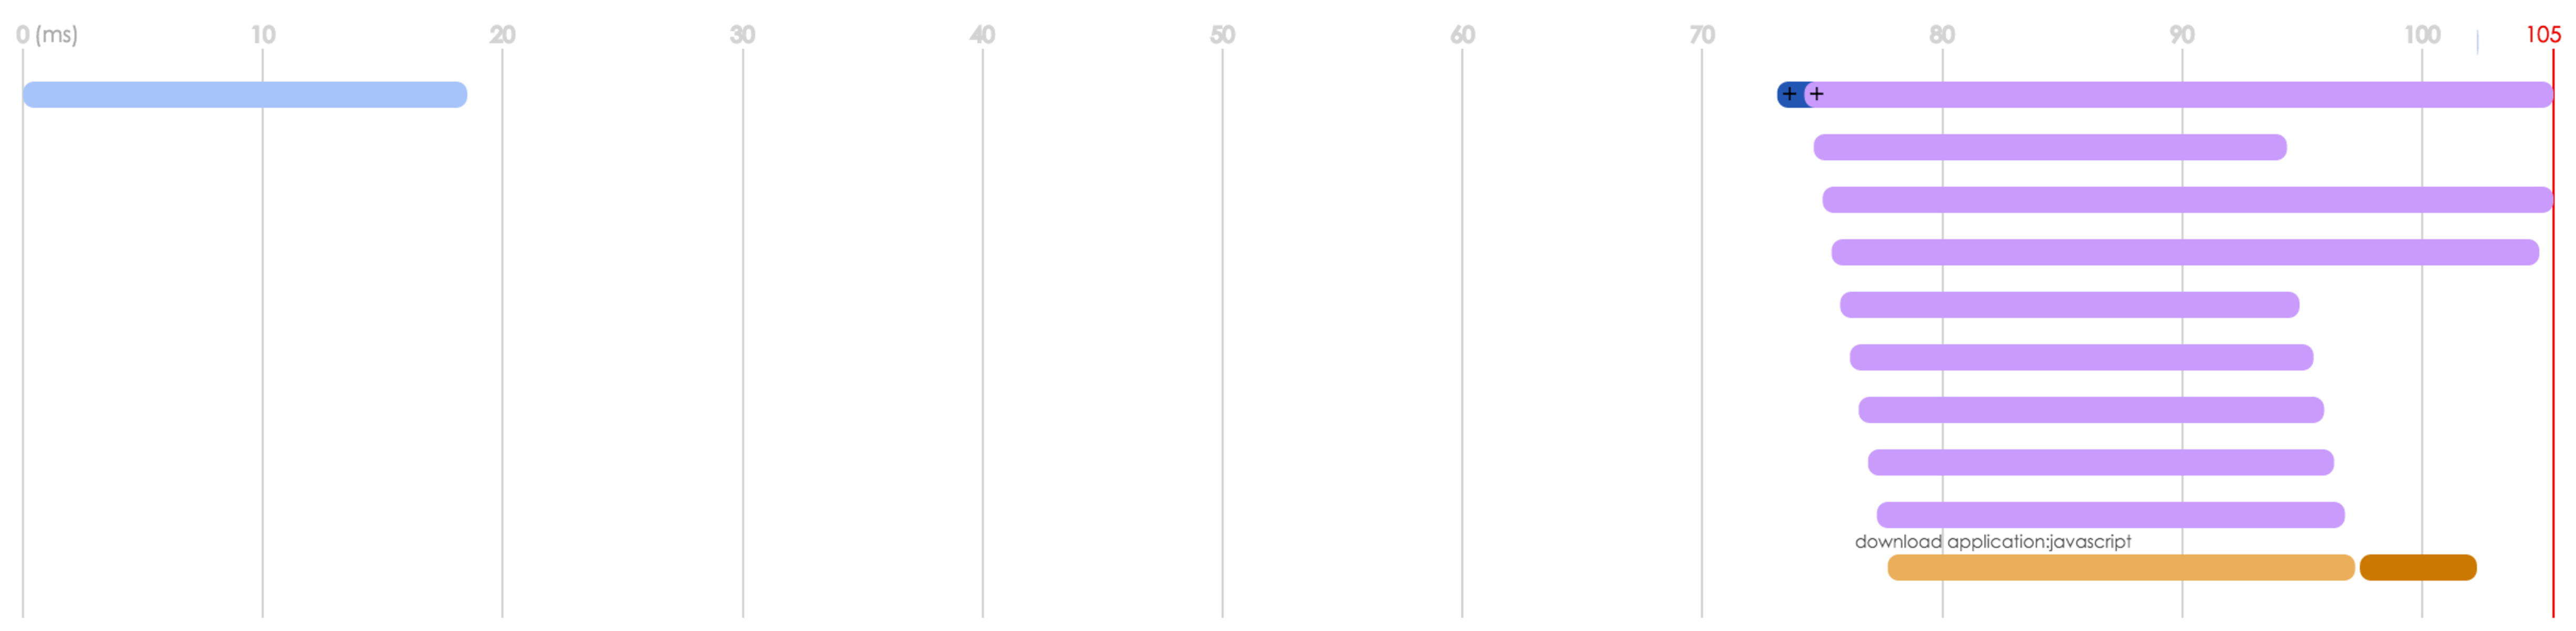
\includegraphics[width=0.85 \textwidth]{./figures/introduction/imagejs.pdf}
  \caption {Dependency graph for a HTML page when Javascript is loaded after all images}
  \label{fig:imagejs}
\end{figure}


  \item Adding Javascript before image load. 
  
  The interesting case is when Javascript code is located before images' ones.
  In this case, when the HTML parser encounters a dynamic activity that needs to be computed and is likely to modify the DOM tree. Browsers block subsequent activities until the dependency relations used in constructing the DOM tree are resolved. 
 If the dynamic activity does affect subsequent activities, It has to be loaded and computed before upcoming ones. 
 
However, in cases where parser realizes that this dynamic activity has no effect on download of subsequent ones, subsequent activities can be safely downloaded shortly after the execution starts .
 
The dependency graph for this scenario is depicted in figure\ref{fig:jsimage}\\
The top bars on the right are showing Javascript ({\em b.js}) download and execution which start before image loads.

  \begin{minted}[frame=leftline, framerule=1.5pt, rulecolor=\color{blue}]{html}
  <html>
  <body>
    <script src = "b.js"> </script>
    <img src = "a.jpg"/>
    <img src = "b.jpg"/>
    <img src = "c.jpg"/>
    <img src = "d.jpg"/>
    <img src = "e.jpg"/>
    <img src = "f.jpg"/>
    <img src = "g.jpg"/>
    <img src = "h.jpg"/>
    <img src = "i.jpg"/>
  </body>
</html>
\end{minted}

 \begin{figure}[!htb]
  \centering
    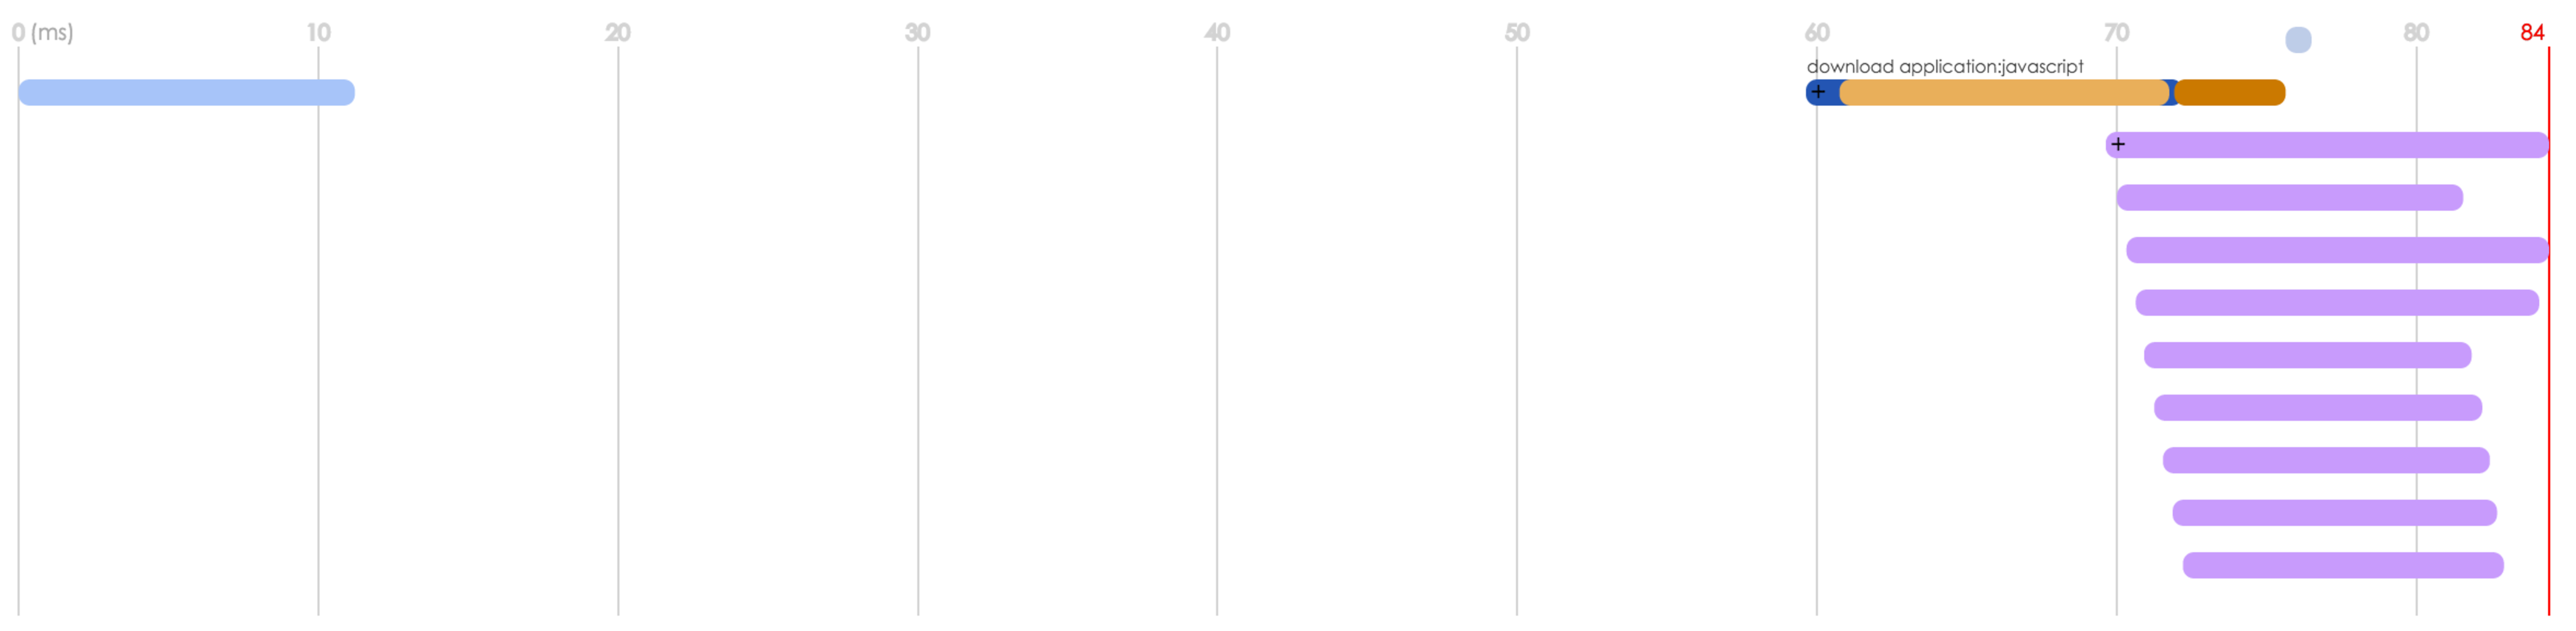
\includegraphics[width=0.85 \textwidth]{./figures/introduction/jsimage.pdf}
  \caption {Dependency graph for a HTML page when Javascript is loaded before images}
  \label{fig:jsimage}
\end{figure}

\end{enumerate}
 We can observe, if we reorder javascript and image locations in an HTML file, the resulting page and consequently the page load time is different.\\
 
\noindent \colorbox{gray!20}{\parbox{0.9\textwidth}{In other words, the performance, depends directly on how the dependency graph between markup, stylesheets, and Javascript is resolved}}

\subsection{Complexity}
The second challenge in improving page load time that we will look into is complexity.
Complexity of a website can be characterized as the number of objects inside it. \\
Adding more objects to a web page structure, not only increases the total size (which naturally means more download and computation time), but also has an effect on complexity of the dependency graph. \\
For instance, adding a Javascript to a page structure, spontaneously imposes one dependency between downloading and execution of that Javascript. Moreover, since Javascript modifies the DOM tree, all subsequent activities need to be blocked until the dependency issues are resolved. 

\noindent In figure \ref{fig:websitegrowth}, each X axis ticks corresponds to a year (J-95 for January 1995) and the right Y axis shows average number of objects for all website analyzes in that particular year.
We can observe that average number of objects in a webpage has doubled in last 7 years. 
The figure \ref{fig:websitegrowth} also shows that size of websites has doubled in only 3 years and 
Although computation power and network bitrate are also increasing, but we are dealing with an ever increasing trend in page size and the average number of objects in a web page. \\

\noindent \colorbox{gray!20}{\parbox{0.9\textwidth}{Increased size and number of objects, in turn, actuates the dependencies inside the page structure.
These all makes improving page load time even more complicated.}}

\begin{figure}[!htb]
  \centering
    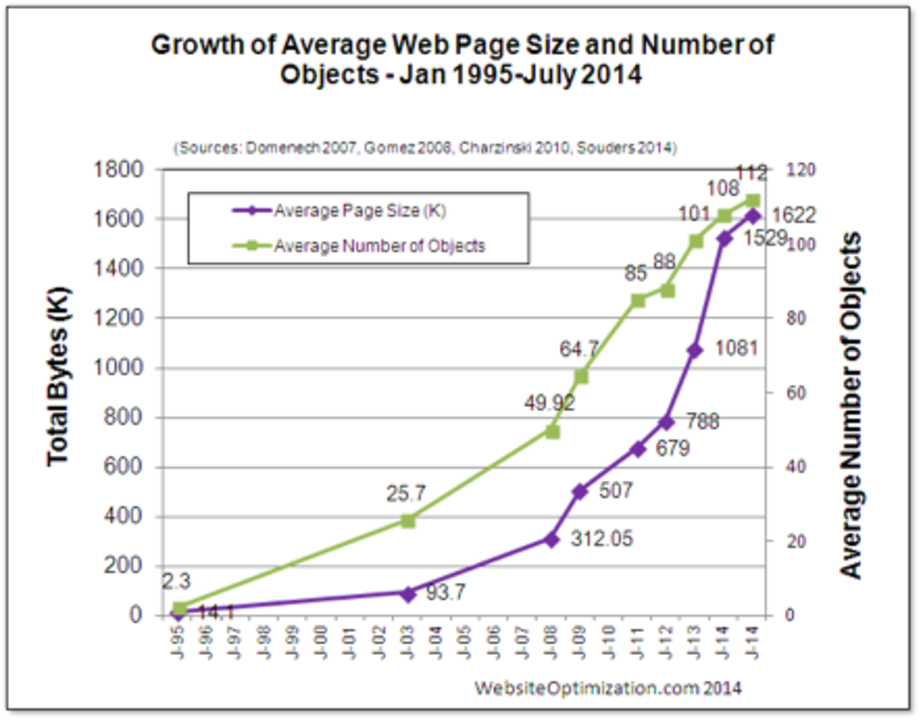
\includegraphics[width=0.75 \textwidth]{./figures/introduction/websitegrowth.pdf}
  \caption {Websites' size and objects growth (source: websiteoptimization.com)}
  \label{fig:websitegrowth}
\end{figure}
\subsection{Variances}
Another challenge that makes studying page load time complicated, is the variability of page load time over wireless/cellular networks. Page load time depends on several factors such as:
\begin{itemize}
\item Underlying network parameters including bandwidth, delay and packet loss.
\item Connection Type can be Wi-Fi, 4G, 3G, \dots, each with different characteristics.
\item Device computation and network resources such as CPU, RAM, wireless chipset,  \dots
 \item Even time and location of access may have effect on quality of network service one receives.
\end{itemize}

\noindent \colorbox{gray!20}{\parbox{0.9\textwidth}{Taking into account all these parameters is not a trivial task.}}

\section{Overview}\label{overview}
%Our goal is to improve Web sites' page load time on mobile devices. We will approach this goal by providing a framework for Web developers that suggest them best optimization applicable to their web sites.
Our primary object is to improve Web page load times. Although there are several approaches to improve Web pages, we propose the following: We will design algorithms and techniques to determine the best optimization(s) for a given page. Our goal is to provide an optimization framework for Web developers that will quickly suggest the best optimizations for a page.

\noindent The remainder of this report is organized as follows.\\
\noindent In order to address dependency and variances challenges, we start off by building a testbed to run our experiments in a controlled environment.
This testbed resolves the variances issue and lets us focus on each varying factor one at a time. (chapter \ref{ch:methodology})\\

\noindent Using the testbed, we first study the characteristics of the mobile page load process. From the experiments ran on this testbed, we observe that although networking time is the main bottleneck in desktop environment, but in mobile environment, main bottleneck in a page load process is the computation time. (chapter \ref{ch:bottleneck})

\noindent However, most mobile optimizations today including FlyWheel\cite{flywheel}, Parcel \cite{parcel}, HTTP/2 \cite{spdy}, attempt to reduce the network latency during page load time. 

\noindent Our dependency graph and critical path analysis approach using this testbed, enables us to study page load time behavior when a certain optimization is applied into a page structure (such as inlining) or when we change the way browsers and servers communicate (for example, enabling compression on server side).\\
\noindent Then, we will employ these findings to build a platform (PLTSpeed, our current project) to suggest users, what optimizations they need to apply and what is the effect of applied optimizations on their page's load time. (chapter \ref{ch:optimization})\\
\noindent In future, we propose to design and build a platform to predict page load time in a fast and scalable manner. Then, using this prediction mechanism, we suggest to users optimization (or an ordered list of optimizations) that most improve their Web site's page load time.\\

%\noindent . (chapter \ref{ch:pltspeed})




